\documentclass{beamer}
\usepackage{tikz}
%\usepgfplotslibrary{external} 
%\tikzexternalize
\usepackage{lmodern}% http://ctan.org/pkg/lm
\usepackage[utf8]{inputenc}
\usetheme{Warsaw}

\title{Missing Values}
\subtitle{A thorn in the side}
\author{Thomas LOUIS}\institute{Data scientist}

\AtBeginSection[]{
  \begin{frame}
  \vfill
  \centering
  \begin{beamercolorbox}[sep=8pt,center,shadow=true,rounded=true]{title}
    \usebeamerfont{title}\insertsectionhead\par%
  \end{beamercolorbox}
  \vfill
  \end{frame}
}


\begin{document}

\begin{frame}
\titlepage
\end{frame}


\section{introduction}
\begin{frame}
	\begin{center}
	\Large Why this presentation ?
	\end{center}
\end{frame}

\begin{frame}
  \begin{tikzpicture}[remember picture,overlay]
   \node[at=(current page.center)] {
     
\includegraphics[width=\paperwidth]{images/22ftbs.jpg}
     };
  \end{tikzpicture}
\end{frame}

% Give examples :
%
% - Poll, people don't answer to every questions => Studies / Research
% - Customer information are rarely complete => recommandation system
% - Technical issues can occur without warnings and you can't recover past data.
% ONE INDUSTRY EXAMPLE
%
\subsection[Missing values in Data Driven Business]{}
\begin{frame}
	Why am I talking about missing values ?
        \begin{enumerate}
		\item<1- | alert@1> Because it's everywhere.
		\item<2- | alert@2> Dealing with missing values is tricky and could lead to disasters  
		\item<3- | alert@3> It's interesting
	\end{enumerate}
\end{frame}

\subsection[Definition of nissing value]{}
\begin{frame}
  \textsc{Missing values}, what is it ?
  \begin{quote}
  Wikipedia : In statistics, missing data, or missing values, occur when no data value is stored for the variable in an observation. Missing data are a common occurrence and can have a significant effect on the conclusions that can be drawn from the data
  \end{quote}
  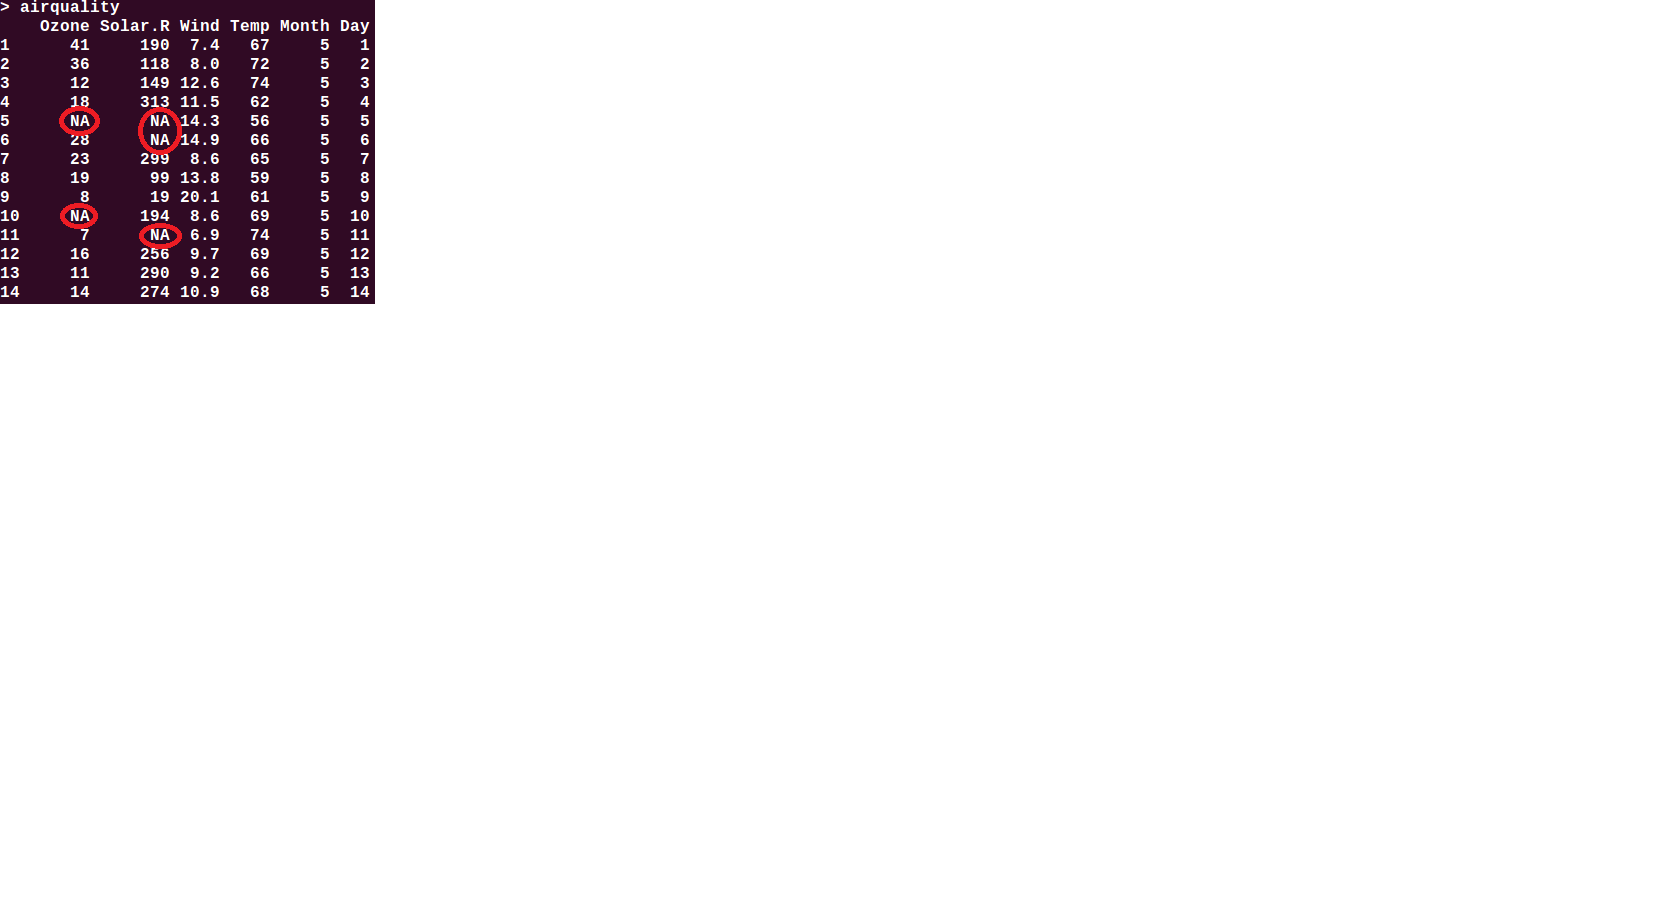
\includegraphics[width=25cm]{images/image_missingvalues.png}
\end{frame}

\section*{Table of content}
	\begin{frame}
		  \tableofcontents[]
	\end{frame}      

\section[A simple case]{A simple case : Clinical trial on different antidepressant}
\subsection{case description}
\begin{frame}
	\begin{itemize}
		\item<1->6 centre clinical trial, comparing 3 treatments of depression
		\item<2->367 subjects randomised to one of 3 treatments
		\item<3->subjects rated on HAMD score (0 to 50)  on 5 weekly visits
		\item<4->Subjects drop out from week 2 onwards (246 complete cases)
		\item<5->Study objectives : compare efficiency of the 3 treatments over time. metric : HAMD
	        \item<6-> Metric : HAMD score changes over the time
	\end{itemize}
\end{frame}

\begin{frame}
  \begin{tikzpicture}[remember picture,overlay]
   \node[at=(current page.center)] {
     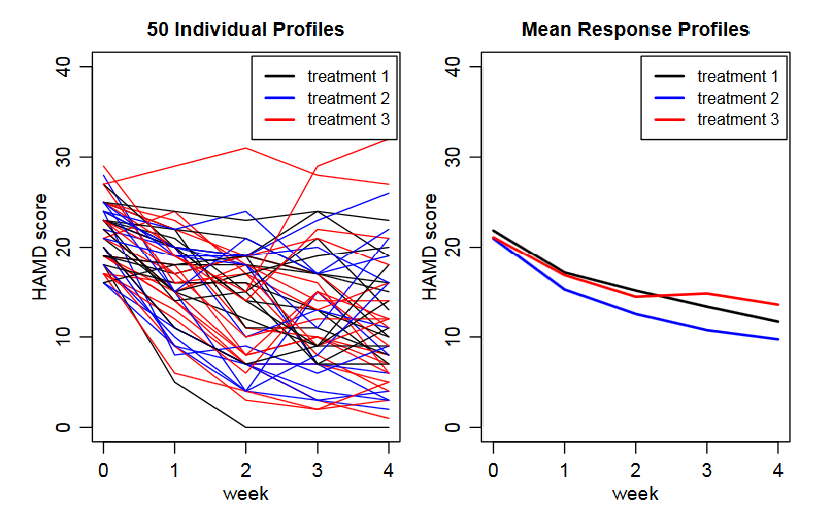
\includegraphics[width=\paperwidth]{images/HAMD_response_profile.png}
     };
  \end{tikzpicture}
\end{frame}

\begin{frame}
  \begin{tikzpicture}[remember picture,overlay]
   \node[at=(current page.center)] {
     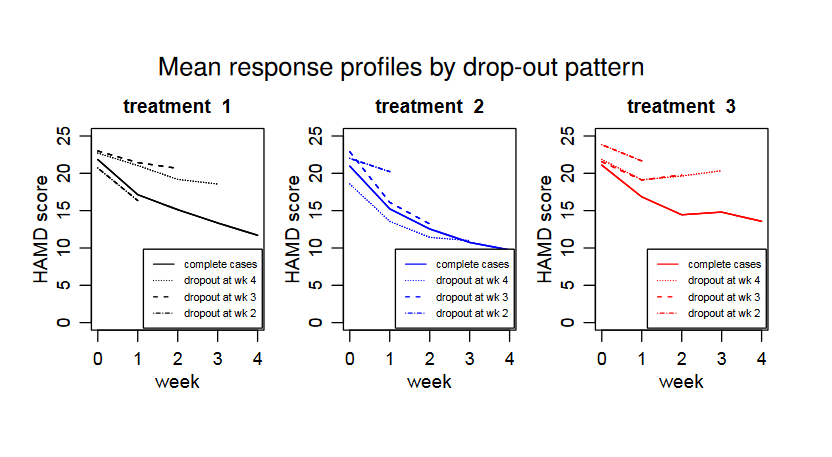
\includegraphics[width=\paperwidth]{images/HAMD_all_response_by_dropout_pattern.png}
     };
  \end{tikzpicture}
\end{frame}



\begin{frame}
\Large How would you proceed ?	
\end{frame}


\subsection{what not to do}
\begin{frame}
Don't drop uncomplete cases
	\begin{itemize}
        \item You will miss the information of 33 \% of individuals 
        \item You make the assumption that the individual that dropout the study are statistically the same than those who don't
	\end{itemize}
\end{frame}

\begin{frame}
Don't replace missing values by last observed values. Even if it is widely used in clinical trials.
	\begin{itemize}
\item It implies strong assumption that treatment doesn't work once individual drop out early. 
\item It also implies that HAMD score will not raise after the individual leave the study. so the result might be better thatn the real effect of the treatment
	\end{itemize}
\end{frame}

\subsection{what to do}
\begin{frame}
	\Large Do something that is statistically not wrong :
	\begin{itemize}
		\item Frequentist
		\item Likelihood 
		\item Bayesian 
        \end{itemize}
        Bayesian approach : prior, likelihood, posterior
\end{frame}

\begin{frame}
	\begin{itemize}
		\item This study using listwise deletion ended up with : 1 \sim 2, 1 \sim 3, 2 \geq 3.
		\item This study using LOCF ended up with 1 \sim 2, 1 \sim 3, 2 \sim 3.
        	\item This study using bayesian analysis ended up with 1 \leq 2, 1 \sim 3, 2 \geq 3.
	\end{itemize}
        \begin{quote}
		"Don't mess with missing data" \textit{Thomas L.}
	\end{quote}
\end{frame}

\section{data science in action}

\subsection{Become a CRISP-DM zealot}
\begin{frame}
        \Large{How to become a CRISP-DM zealot}
	\textbf{Cross Industry Standard Process for Data Mining}
	\begin{enumerate}
		\item<1- | alert@1> Business Understanding 
		\item<2- | alert@2> Data understanding + KPI definition 
		\item<3- | alert@3> Modeling (start with a baseline) 
		\item<4- | alert@4> Evaluation  
		\item<5- | alert@5> Iterate 4-5 Until KPI are reached 
		\item<6- | alert@6> Deployment  
		\item<8- | alert@7> Monitoring 
	\end{enumerate}
\end{frame}

\subsection{Understanding data}
\begin{frame}
        \textbf{Understanding data}
	\begin{itemize}
		\item<1- | alert@1> Why is it missing ? 
		\item<2- | alert@2> Is it really missing ?  
		\item<3- | alert@3> "Nan" may not be the only missing data
	\end{itemize}
\end{frame}

\begin{frame}
	\textbf{Let's talk about missingness}
	\begin{itemize}
		\item<1- | alert@1> MCAR : P(R \vert Y_m,Y_o,X) = P(R) 
		\item<2- | alert@2> MAR : P(R \vert Y_m,Y_o,X) = Pr(R \vert Y_o,X)
		\item<3- | alert@3> CDM : P(R\vert Y_m,Y_o,X) = P(R \vert X) 
                \item<4- | alert@4> MNAR : none of them
	\end{itemize}
\end{frame}

\begin{frame}
        \textbf{How to test it ?}
	\begin{itemize}
	\item MCAR : little's \chi^2 test, R's mcartest package
        \item MAR : your nose, or more information
        \item CDM : little's \chi^2 test, R's mcartest package
	\end{itemize}\\
        \textbf{How little's test work ?}\\
        H_0 : y_o_i\vert r_i \sim N(\mu,\sigma)\\
        H_1 : y_o_i\vert r_i \sim N(\alpha,\beta)\\
\end{frame}


\subsection{Data preparation and modeling}
\begin{frame}
\textbf{What do i do now ?}
\begin{itemize}
\item listwise deletion if required assumption are verified 
\item make a model that is able to handle missingness : feature enginerring
\item perform simple/multiple imputation
\item do nothing : don't waste time if it's impossible
\end{itemize}\\
Don't forget that you are not in a Kaggle competition, you can invest money to recover missing values
\end{frame}

\section{Multiple Imputation}
\begin{frame}
\textbf{An art of playing with fire : generating data from void}\\
There are different technics as it is an open research subject
\begin{itemize}
\item MICE : simple, handy, good empirical results, but lacks of theoritical background   
\item Bayesian approches : theoriticaly and praticaly state of the art
\item Autoencoder/decoder NN : fancy but no theoritical background
\end{itemize}
\end{frame}

\subsection{MICE}
\begin{frame}
  \begin{tikzpicture}[remember picture,overlay]
   \node[at=(current page.center)] {
     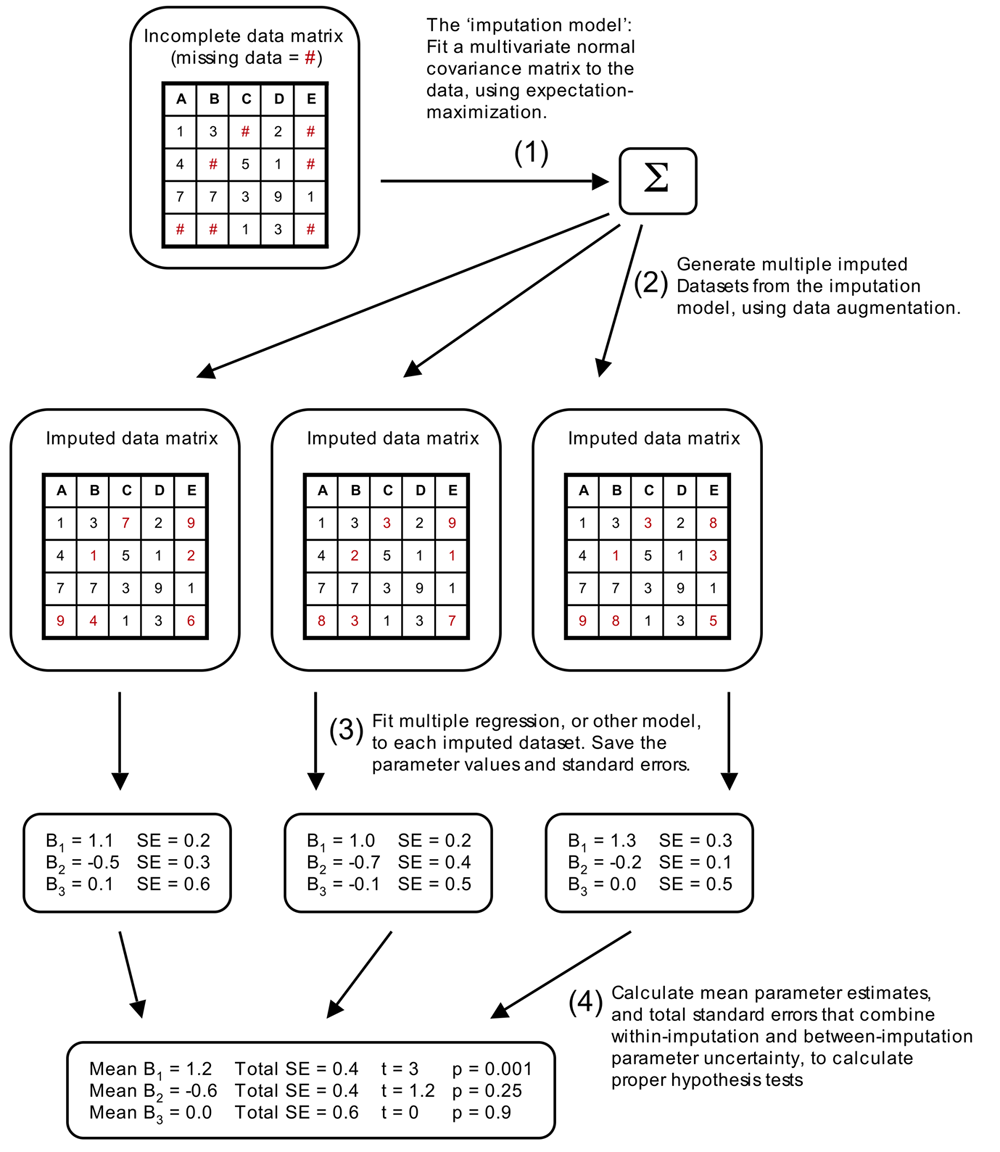
\includegraphics[width=\paperwidth,height=\paperheight,keepaspectratio]{images/MICE.png}
     };
  \end{tikzpicture}
\end{frame}


\subsection{Bayesian apporach}
\begin{frame}
  \begin{tikzpicture}[remember picture,overlay]
   \node[at=(current page.center)] {
     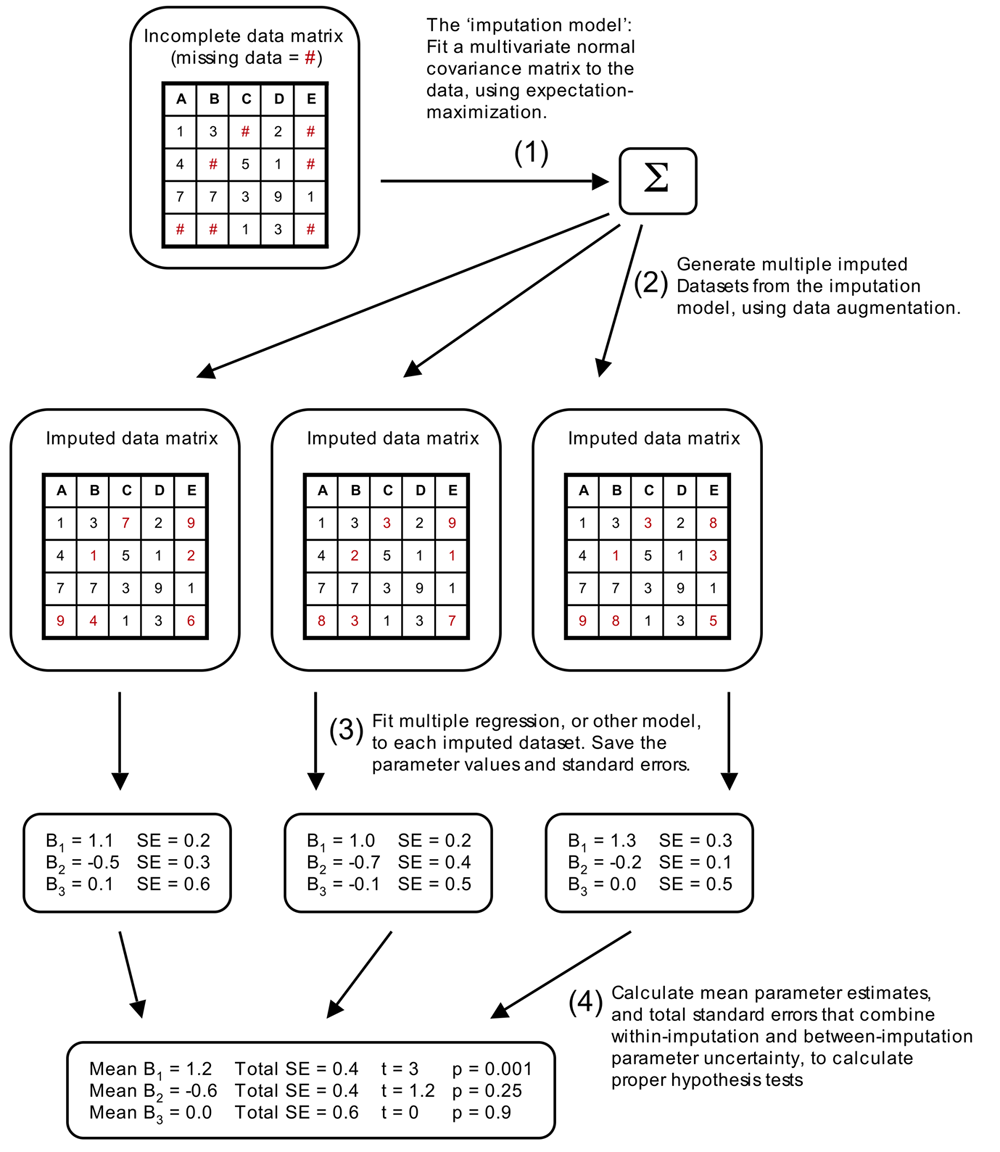
\includegraphics[width=\textwidth,height=\textheight,keepaspectratio]{images/MICE.png}
     };
  \end{tikzpicture}
\end{frame}

\section{Conclusion}
\begin{frame}
\end{frame}

\section{references}
\begin{frame}
	\begin{itemize}
		\item Constructing Models to Deal With Missing Data | SciPy 2016 | Deborah Hanus, https://www.youtube.com/watch?v=cHzahWjaA7o
                \item http://www.bias-project.org.uk/papers/NonTechnicalMissingTalkSlides.pdf
                \item http://www.stata-journal.com/sjpdf.html?articlenum=st0318
                \item https://www.linkedin.com/pulse/imputing-missing-data-playing-fire-jehan-gonsal/?trackingId=R3Li3WglgwDRafeF95nAJw%3D%3D
	\end{itemize}
\end{frame}


\end{document}

% some references :
% - Constructing Models to Deal With Missing Data | SciPy 2016 | Deborah Hanus, https://www.youtube.com/watch?v=cHzahWjaA7o
% - http://www.bias-project.org.uk/papers/NonTechnicalMissingTalkSlides.pdf
% - http://www.stata-journal.com/sjpdf.html?articlenum=st0318
